\subsection{background: scheduling}

Tor handles multiple queues of cells for each circuit and writes cells in the
outbound connection while favoring bursty over bulky traffic. The main idea is
to prioritize circuit handling interactive data streams, like chats or web
browsing. Tor uses an heuristic called EWMA~\cite{tang2010improved} (i.e.,
computes the exponentially weighted moving average for the number of cells sent
on each circuit) to decide which circuit to prioritize. Recently, the efficiency
of EWMA has been improved with the Kist~\cite{jansen2014never} scheduler used to
reduce the congestion on the kernel outbound queue and push back this delicate
problem on to the Tor layer.

In an ideal network, we might expect that traffic movement is an exclusive
function of the raw bandwidth capacity in each edge connection and the
scheduling algorithm implemented at each node.  The Tor network employs EWMA to
favor interactive web clients over continuous bulk clients. In moneTor, we
originally proposed to modify EWMA with a simple linear scaling factor that
would favor paid circuits.
%\begin{equation}
%  A_{t + \Delta t} = A_t \times 0.5^{\Delta t/H}
%\end{equation}
%\begin{equation}
%  A'_{t + \Delta t} = A_{t + \Delta t} / \beta + C_{t, t + \Delta t}
%\end{equation}
%Defined in Tang and Goldeberg's original paper~\cite{tang2010improved}, $A$ is a variable score used to
%sort circuits such that the circuit with the lowest $A$ is always next on the
%scheduling queue. $C$ is the number of cells relayed within $\Delta t$, the time
%since the previous observation, and $H$ is a global representing the half-life
%decay interval in the score. Our added term, $\beta \in [1, \inf)$, is a tunable
%parameter such that $Bandwidth_{premium} = Bandwidth_{nonpremium} \times \beta$
%for any given circuit under ideal conditions.

\subsection{Obstacles}

Implementation into the concrete Tor infrastructure has proven to be a
considerably more complex problem. Upon failing to achieve meaningful
differentiation with low values of $\beta$, we adopted a more blunt policy which
\emph{always} services premium circuits first and implemented it in a
zero-overhead version of moneTor.\footnote{This ideal version of moneTor strips
  away all payment operations and instead passes a single signal through the
  network to distinguish premium circuits.} The results are displayed in
Figure~\ref{fig:scheduling_priority}. Although we observed some moderate
differentiation, the difference falls well short of the benefit needed to
incentivize paid users as well as our expectations for such an inequitable
scheduling policy. This result holds even under very heavy levels of induced
congestion.

This is a severe issue since all previous works are using strategies that
make local scheduling decisions on each relay to serve premium bandwidth.
We observe that offering bandwidth priority based on local decisions seems not
to work well anymore.

\begin{figure} \centering
  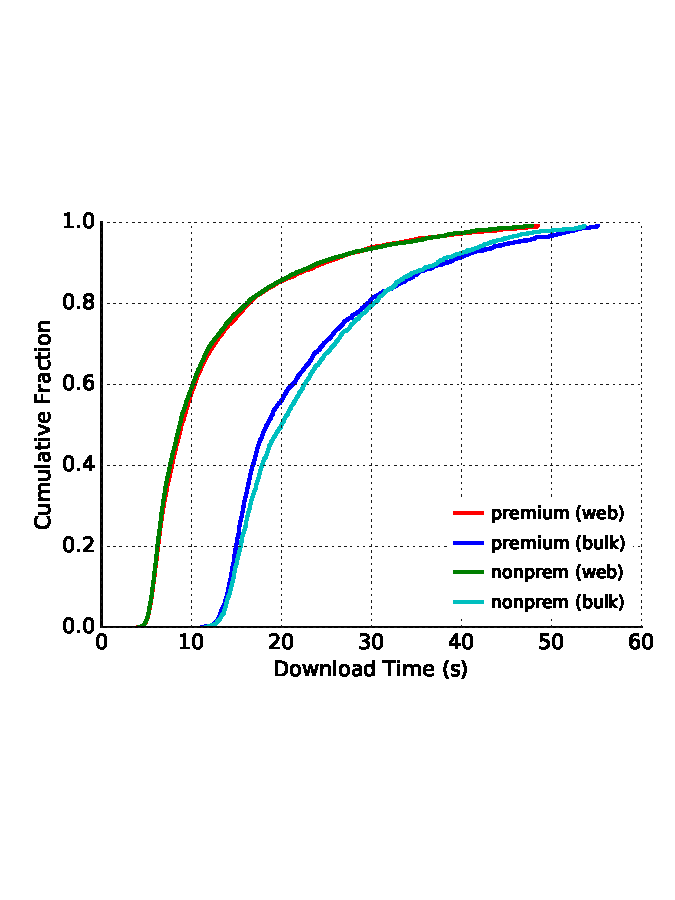
\includegraphics[trim={0 3cm 0 3cm}, clip, width=0.32\textwidth]{images/scheduling_priority.pdf}
  \caption[Prioritized Scheduling]{Prioritized Scheduling --- CDF download
    times for superimposed web and bulk clients where premium status is enforced
    only via scheduling. Almost no priority is observed.}
  \label{fig:scheduling_priority}
\end{figure}

\subsection{Investigation and discussion}

Our negative results can be explained if scheduling is not the most decisive
determining factor in performance. To verify this hypothesis, we studied the
incoming queue from which the scheduler is able to select new active
circuits. Figure~\ref{fig:scheduling_far} illustrates the temporal load in the
queue at a single exit relay over a one-minute time span. The height of the
curve represents the total number of cells waiting to be serviced at each
continuous point in time while the colors group quantities of cells that belong
to the same circuit. Figure~\ref{fig:scheduling_close} displays a subset of the
same information within a smaller time interval.\footnote{While the graph has
  the visual appearance of a bar graph, this is just a function of the striking
  data pattern. In actuality, the plot displays a stacked area graph.} In the
aforementioned figures, notice that the queue is only populated for a period of
10 $ms$ before it is completely flushed, implying the queue spends the vast
majority of its time empty. This 10 $ms$ window is a product of Tor's internal
event handling framework and is consistent with data from Jansen et
al~\cite{jansen2018kist}. We found in an analysis of the line-by-line
observations of the queue activity that while cells are flushed in the correct
order, they appear in the queue at roughly equal proportions. In effect,
bandwidth in our simulation is not constrained by the ordering policy of the
scheduler but rather by the rate at which they arrive from the network. As a
consequence, local decisions at a particular relay for scheduling falls short
to offer the expected priority. Note that the same problem was already spotted by Jansen \textit{et al.}~\cite{jansen2018kist} which motivated the deployment of KIST. Our results show that despite the use of KIST, relays may still be able to flush all queues at once, dismissing the effect of the scheduler's choice. 


\begin{figure} \centering
  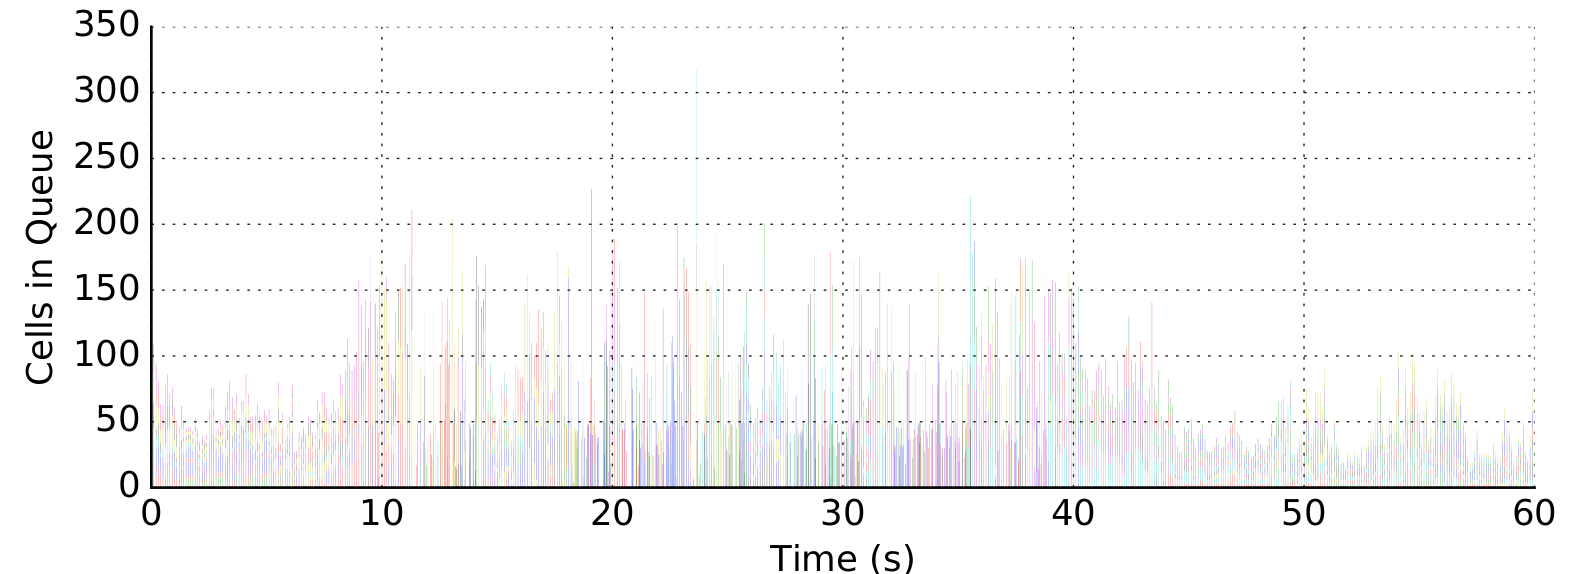
\includegraphics[width=0.49\textwidth]{images/scheduling_far.png}
  \caption[Queue Temporal Profile (60 seconds)]{Queue Temporal Profile
      (60 seconds) --- Size of the scheduling buffer over time at a single exit
    relay in terms of number of cells. Colors group cells belonging to the same circuit.}
  \label{fig:scheduling_far}
\end{figure}

\begin{figure} \centering
  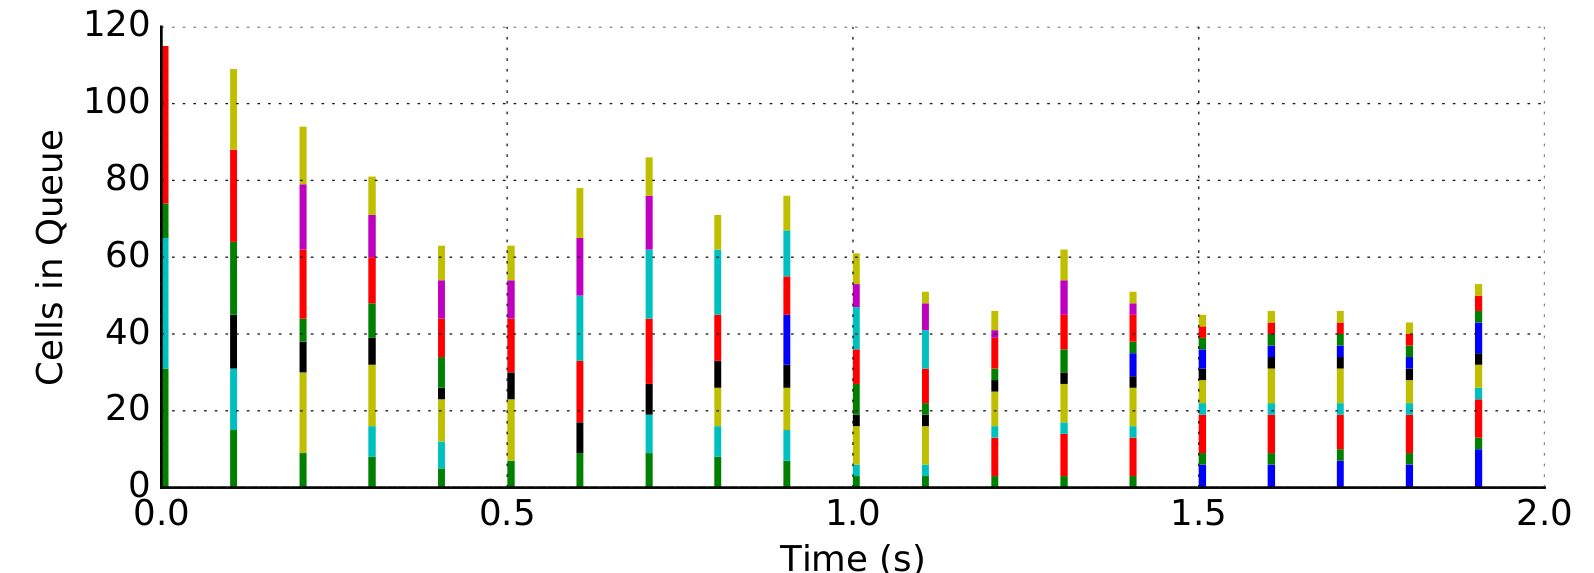
\includegraphics[width=0.49\textwidth]{images/scheduling_close.png}
  \caption[Queue Temporal Profile (2 seconds)]{Queue Temporal Profile
      (2 seconds) --- Size of the scheduling buffer over time at a single exit
    relay in terms of number of cells. Colors group cells belonging to the same
    circuit.}
  \label{fig:scheduling_close}
\end{figure}

Now, we may investigate why this situation happens over our simulations while prioritization based on making decisions inside the 
relay's scheduler worked fine for previous works such as BRAIDS and LIRA while we 
follow the same methodology to evaluate moneTor. So, what could be wrong? First, 
it may be the case
that other network control mechanisms within the Tor codebase constrain the flow
of cells, rendering the mostly idle scheduler to be ineffective. This may be
caused by any combination of factors including point-to-point flow control,
connection throttling, or some less documented threshold embedded in the
code. Yet, we believe that some differences in the code could not explain our 
results for the following reason: our positive results covered in Section~
\ref{sec:priority_exp} showing
increasing performance (resp. decreasing) when we increase (resp. decrease) the 
circuit windows are counter-intuitive compared to previous works exploring the 
effect of changing the window sizes~\cite{archive-2009-mail, kiraly2008solving, 
dingledine2009performance}, and Tor's code covering those aspects did not change 
meaningfully for many years. This is an interesting piece of information, and we 
expect these results to be linked to our actual 
problem of not achieving to prioritize flows based on relays' scheduler decision.

To explain those oddities, we found and verified the following reason: the 
constraining network bottleneck has moved from the
Tor network itself to the exit relay interface with external servers on the
web. In this scenario, cell queuing within Tor is not nearly as important as the
TCP/IP packet handling at each exit relay. Actually, both approaches to prioritize 
flows are complementary: when the congestion is inside the Tor network, applying 
local scheduling policies makes an efficient priority mechanism as demonstrated by previous works. Also in such a situation, priority 
based on the flow-control (that is, a function of the global circuit) would not be 
efficient, because all cells would spend the majority of the time waiting in 
relays' FIFO queues anyway. In the opposite, if the congestion is outside the Tor 
network (between the exit relays and the destination), then local scheduling 
policies would fall short to make any prioritization as showed in Figure~\ref{fig:scheduling_priority}, but priority based on the 
flow-control would achieve to prioritize flows, as demonstrated in Section~\ref{subsec:experiments}. 

The shift of congestion from the internal Tor network to the exit gateways explains why our scheduling results in Figure~\ref{fig:scheduling_priority} are different from BRAIDS
and LIRA. Indeed, BRAIDS run experiments with Tor version \texttt{0.2.0.35} and a network history
from January 2010~\cite{braids-repository}. This Tor version's commit is
before a major change in the path selection mechanism that reduced Tor's
internal congestion problem and greatly improved the performance. This major change
was introduced as the bandwidth-weights in Mike Perry's commit \texttt{0ff86042ac16}
dated from September 2010. The bandwidth-weights are a set of weights specified
in the directory specifications, section 3.8.4~\cite{dirspec}, that aim at
balancing the overall network usage. Those weights are
critical for the network performance, and also for
anonymity~\cite{waterfilling-pets2017, wf_proposal}. Importantly, the benefit
of Mike Perry's bandwidth-weights are proportional to the inequalities between
the overall bandwidth in circuit positions. These inequalities are growing fast for years, as we can observe in Figure~\ref{fig:bw_inequalities}.
%In consequences, compared to BRAIDS's experiments which use a non-balanced path selection and a old internally congested network, our moneTor experiments are no more in a situation
%where we have a lot of internal congestion, and we cannot achieve the same
%priority improvement using a local scheduler at each relay.

\begin{figure}
  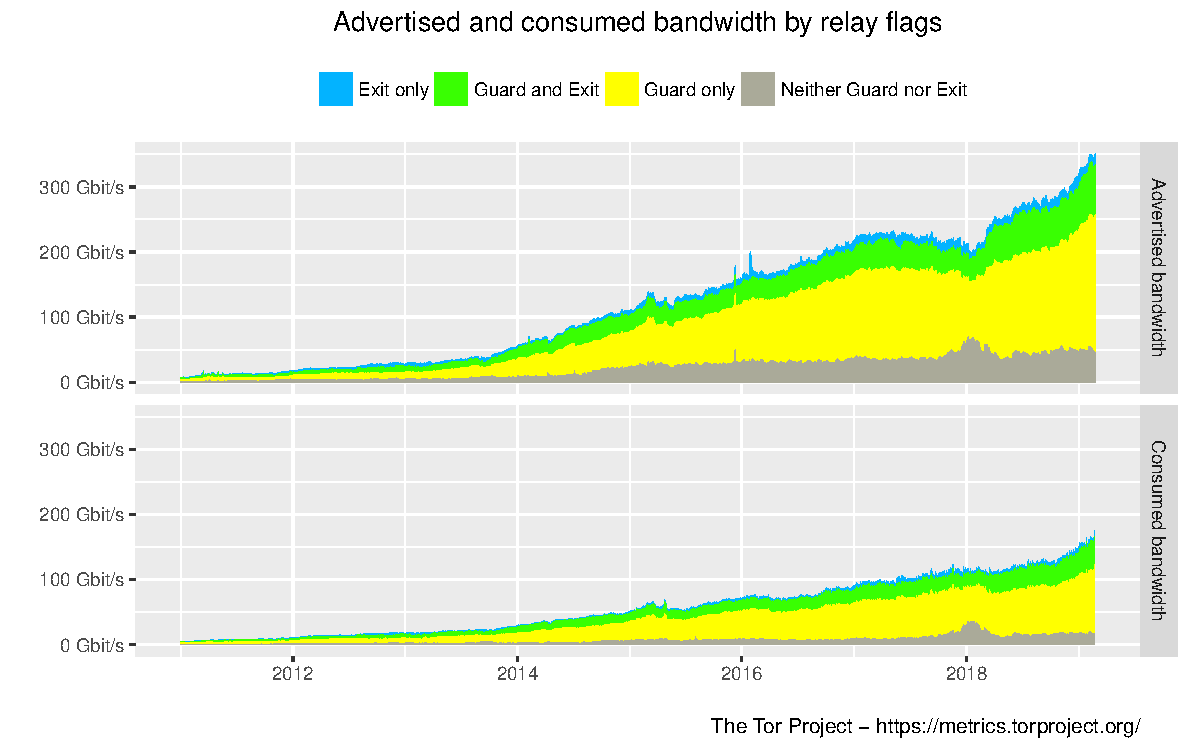
\includegraphics[scale=0.415]{images/bandwidth-flags-2011-01-01-2019-02-25.pdf}
  \caption{Evolution of bandwidth aggregated by relay flags} \label{fig:bw_inequalities}
\end{figure}

LIRA's experiments are based on \texttt{tor-0.2.3.13-alpha} from March 2012, which benefits
from Mike Perry's bandwidth-weights. This may explain why LIRA has less impressive priority advantage than the one exposed in BRAIDS: experiments in LIRA are probably less internally congested than the ones from BRAIDS, and a major change in the path selection to solve a performance problem seems to bear some responsibilities for this case. However, the different congestion status may also be due to other factors, such as a different client usage model and the local scheduling policies. Comparing to our experiments, LIRA uses a simulated environment scaled down from an April 2012 consensus with $\approx 42\%$ of relays with the \texttt{Exit} flag, while our experiments only have $\approx 13\%$ of relays with the \texttt{Exit} flag. This is a consequence of the state of the Tor network from which Shadow simulations are built. The difference in the state of the Tor network may also be observed on Figure~\ref{fig:bw_comp}, where we plotted the distribution of bandwidth allocated to each position. LIRA's experiments were performed when the exit capacity of the Tor network was not scarce. This is not the case anymore as observed for moneTor's used consensus. This result holds now since a few years~\cite{waterfilling-pets2017}.


\begin{figure}
	\centering
  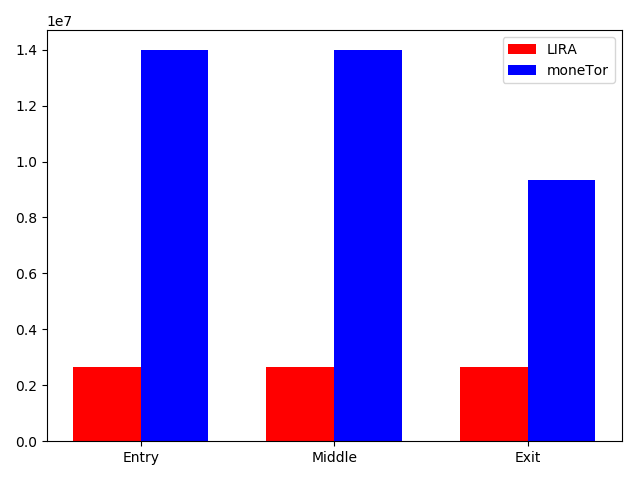
\includegraphics[scale=0.415]{images/bw_analysis_comp.png}
  \caption{Bandwidth distribution in consensuses used for BRAIDS, LIRA and moneTor experiments - BRAIDS does not benefit from bandwidth-weights to refill Middle, LIRA benefits from bandwidth-weights to offer balance between all positions, moneTor benefits from bandwidth-weights to balance entry and middle, yet does not have enough exit nodes to achieve the full balance} 
  \label{fig:bw_comp}
\end{figure}

 
To summarize, as the network grows to offer a lot of internal bandwidth (Figure~\ref{fig:bw_inequalities}, Figure~\ref{fig:bw_comp}), LIRA and BRAIDS's schedulers would tend to become less efficient for providing priority, as demonstrated in our experiments and showed in Figure~\ref{fig:scheduling_close}. 
We must emphasize that we argue for a tendency: our results are no way indicative of the exact same state of affairs for all relays in the real Tor network. The aforementioned experiments
were performed on a considerably smaller scale than the real Tor network with simplistic models for
network topology and user behavior. What can be said is that networking as a
whole is an immensely complex and unpredictable domain and that the attainment
of a simulation environment conducive to effective scheduling is, at the very
least, nontrivial. Consequently, we could argue that the barrier to deploy monetary incentives is not only a social barrier. We may not be ready on a technical level, and technical properties of the scheme may influence social aspects. We showed in this work to be able to offer novel technical properties such as a payment system that scales with trustless entities and fair-exchange (i.e., you pay for what you use), maybe other desirable properties remain to be discovered? Moreover, further research should be conducted to find an ideal priority mechanism that covers various
aspect of circuit congestion. We leave the design of a new priority-based scheme which takes those aspects in account as a further work.

%To confirm it, we run highly congested simulations with many more Tor clients
%than what the scaled-down Tor network could reasonably handle, and observed
%the same results: we were not able to achieve meaningful flow priority with
%local scheduling decisions, but only by tweaking the flow-control mechanism.
